\pagebreak
\subsubsection{UC49-Avvia chat}
\begin{figure}[h] 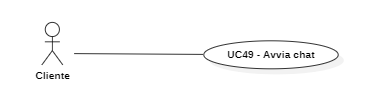
\includegraphics[scale=1]{uc49.png} \end{figure}
\begin{itemize}
\item \textbf{Attore principale:} Cliente.
\item \textbf{Precondizioni:} Il cliente è nella pagina di visualizzazione di un ristorante.
\item \textbf{Postcondizioni:} Diventa possibile comunicare con il ristoratore.
\item \textbf{Scenario principale:}
\begin{enumerate}
    \item Il cliente ha dei dubbi che vuole chiarire;
    \item Il cliente preme il bottone di avvio della chat;
    \item Il sistema crea la chat;
    \item Viene visualizzato un bottone di apertura della chat al posto dell'avvio chat;
    \item Diventa possibile comunicare bidirezionalmente tra il cliente e il ristoratore.
\end{enumerate}
\end{itemize}

\subsubsection{UC50-Apertura chat}
\begin{figure}[h] 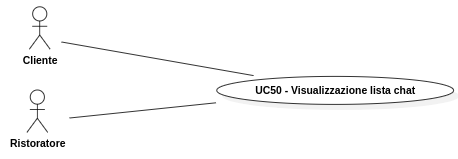
\includegraphics[scale=1]{uc50.png} \end{figure}
\begin{itemize}
\item \textbf{Attore principale:} Cliente / Ristoratore.
\item \textbf{Precondizioni:} Il cliente ha avviato la chat.
\item \textbf{Postcondizioni:} L'attore principale visualizza i messaggi.
\item \textbf{Scenario principale:}
\begin{enumerate}
    \item L'attore principale vuole visionare i messaggi in chat o inviare ulteriori messaggi;
    \item L'attore clicca sul tasto della chat;
    \item Diventa possibile interagire con la chat.
\end{enumerate}
\end{itemize}

\textbf{UC50.1-Invio messaggio}
\begin{itemize}
\item \textbf{Attore principale:} Cliente / Ristoratore
\item \textbf{Precondizioni:} È stata aperta la chat.
\item \textbf{Postcondizioni:} È stato inviato il messaggio.
\item \textbf{Scenario principale:}
\begin{enumerate}
    \item L'attore principale scrive il messaggio nella barra di testo messa a disposizione;
    \item L'attore preme il bottone di invio;
    \item Il messaggio viene salvato nel database in forma criptata;
    \item Il/i destinatario/destinatari ricevono i messaggi.
\end{enumerate}
\end{itemize}

\textbf{UC50.2-Lettura messaggio}
\begin{itemize}
\item \textbf{Attore principale:} Cliente / Ristoratore
\item \textbf{Precondizioni:} È stata aperta la chat.
\item \textbf{Postcondizioni:} I messaggi sono visualizzati a schermo.
\item \textbf{Scenario secondario:}
\begin{enumerate}
    \item L'attore principale deve aver aperto la chat;
    \item Il sistema scarica i messaggi criptati dal database;
    \item Il sistema decripta i messaggi e li visualizza a schermo.
\end{enumerate}
\end{itemize}
